\subsection{Operacje na mapach bitowych}
\label{subsec:operacje-na-mapach-bitowych}

\subsubsection{Generowanie ruchów piona}

Pion ma do dyspozycji parę możliwych ruchów, które należało zaimplementować: ruch o~jedno pole do przodu, ruch o dwa pola do przodu, bicie w lewo, bicie w prawo oraz ruch en-passant.
Każdy z graczy zaczyna rozgrywkę z ośmioma pionami, a w większości partii ich ilość pozostaje znaczna aż do zakończenia rozgrywki.
Czasochłonna wydawała się więc iteracja po~wszystkich bierkach tego typu i indywidualne generowanie ruchów dla każdego z osobna.
Z tego względu wykorzystano operacje bitowe i przesunięcia na masce bitowej.

Poniżej przykład generowania ruchów dla białych pionków.
\begin{align*}
    moves & = empty && \text{pole końcowe musi być puste} \\
    moves & = moves \wedge (P_w\ll16) && \text{pionek musi być dwa wiersze niżej}\\
    moves & = moves \wedge (empty\ll8) && \text{wiersz niżej musi być pusty}\\
    moves & = moves \wedge rank4 && \text{pole końcowe musi być w czwartym wierszu}
\end{align*}

\begin{figure}[ht]
    \centering
    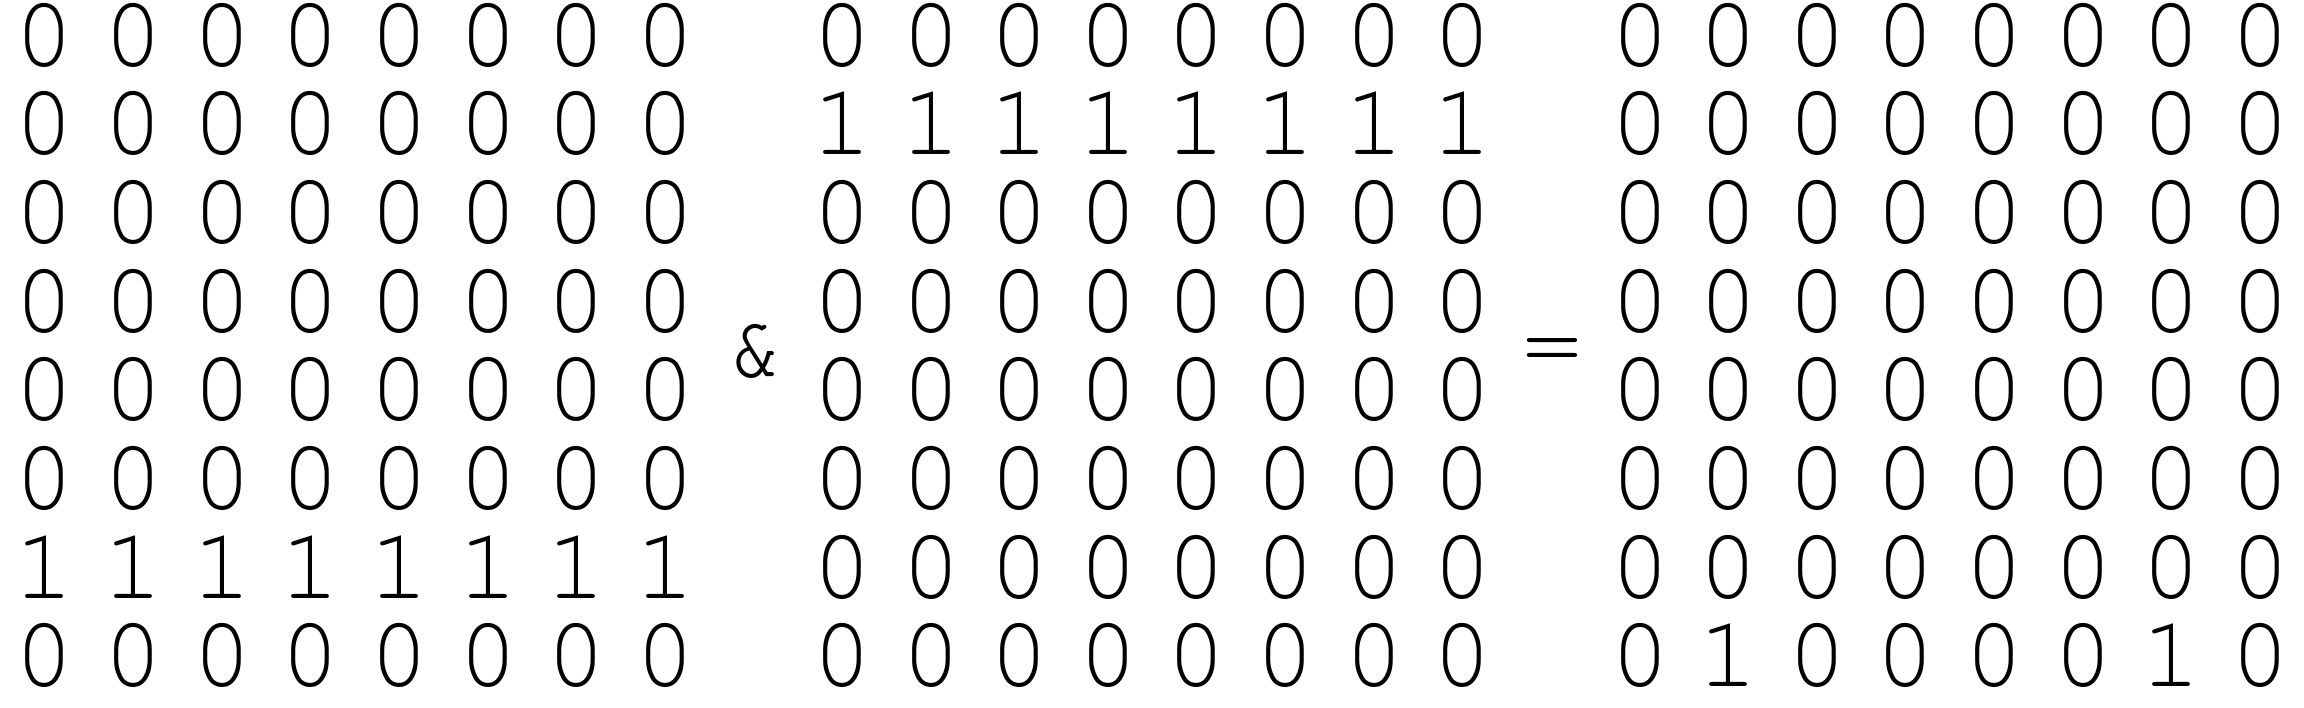
\includegraphics[width=0.85\linewidth]{rozdzialy/rozdzial01/3_generowanie-ruchow/rysunki/bitboards-arithmetic}
    \caption{Kodowanie ruchu szachowego}
    \label{fig:bitboards-arithmetic}
\end{figure}


\subsubsection{Generowanie ruchów hetmana, wieży i gońca}

Ruchy hetmana są połączeniem ruchów wieży oraz gońca, z tego względu można je generować w ten sam sposób.
Techniki te operują na bardzo podobnych zasadach, co generowanie ruchów piona, z tą różnicą, że figury mogą poruszać się o dowolną liczbę pól w danym kierunku, aż do momentu napotkania innej bierki na swojej drodze.
Aby uniknąć skomplikowanych obliczeń, należało zaimplementować funkcję, która w literaturze znana jest pod nazwą (ang.~\emph{Hyperbola Quintessence}).

$lineAttacks =   (o-2r) \string^ reverse( o'-2r')$

\subsubsection{Generowanie ruchów króla i skoczka}

